\documentclass[10pt, a4paper]{IEEEtran}
\usepackage[T1]{fontenc}
\usepackage{mathtools}
\usepackage[usenames,dvipsnames]{color}
\usepackage{parskip}
\setlength{\parskip}{0pt}
\setlength{\parindent}{15pt} 
\usepackage{multirow}
\usepackage{amsfonts}
\usepackage{mathtools}
\usepackage{booktabs}
\usepackage{listings}
\usepackage[justification=centering]{caption}
\usepackage{pgfplots}

\title{Software Optimizations for Reduced CPU Energy Consumption: A Feasibility Study}                            
\author{\IEEEauthorblockN{Stephen I. Roberts and Stephen Jarvis} \\
\IEEEauthorblockA{Department of Computer Science,\\
The University of Warwick}\\
\and 
\IEEEauthorblockN{Chris January and Jonathan Byrd} \\
\IEEEauthorblockA{Allinea Software}}                                                            

\hyphenation{scaling}

\newcommand{\golden}{}
%\renewcommand{\golden}{{\color{green} \checkmark}}


\newcommand{\findref}{}
\renewcommand{\findref}{{\color{red} FindRef}}

\newcommand{\todo}[1]{}
\renewcommand{\todo}[1]{{\color{red} TODO: {#1}}} % comment me out for prod

\newcommand{\reword}[1]{}
\renewcommand{\reword}[1]{{\color{blue} Reword: {#1}}} %

\newcommand{\fragment}[1]{}
\renewcommand{\fragment}[1]{{\color{green}<fragment>}{#1}{\color{green}</fragment>}} %

\makeatletter
\newcommand{\choice}[2][ |]{{\color{Purple}\{%
  \def\nextitem{\def\nextitem{#1}}%
  \@for \el:=#2\do{\nextitem\el}%
\}}}
\makeatother

\begin{document}                                                                
\maketitle

\begin{abstract}
Reducing energy consumption is a prerequisite for future advances in computing at scale. This fact has led performance engineers to look towards software-level power optimization as a potential means to reduce the energy consumed by scientific codes. We present an investigation into the feasibility and potential benefits of this approach. We assess various power measurement and modelling techniques and comment on their ability to help developers identify power optimizations. We then attempt to provide a realistic idea of how much benefit can be expected as a result of applying these optimizations. We find that for current hardware there is limited scope for improving energy efficiency through software optimisation alone. \golden
\end{abstract}

\section*{Introduction \golden}
Driven by Moore's Law, advances in processor design have delivered improvements in CPU performance for decades. As physical limits are reached, however, refinements to the same basic technologies are beginning to show diminishing returns. One side-effect of this is an unsustainable rise in system power use, which the US Department of Energy has identified as a primary constraint for exascale systems \cite{shalf:2011aa}. \golden

Hardware manufacturers are increasingly prioritising energy efficiency in their processor designs~\cite{kurd:2014aa}. In turn, some groups expect that software modifications will be required to fully exploit energy efficiency improvements in modern processors~\cite{shao:2013aa}. They suggest this process will be analogous to the current practice of tuning code to reduce runtime.

%This is analogous to the current practice of tuning code for reduced runtime by exploiting specific processor features like vectorisation or the cache hierarchy. These groups expect code optimisation to be applied to minimizing power consumption as well as run time in the future. \golden

%A body of research is accumulating as the search for techniques to identify and reason about software power optimizations continues.

This paper attempts to provide a critical review of the field; identifying the opportunities present and the amount of benefit which they offer. Our ultimate aim is to help performance engineers make an informed choice when deciding where focus their optimization efforts. To this end we derive a simple yet informative heuristic model of the benefits a given code can expect from power optimization. We then then undertake an empirical investigation in which we apply techniques proposed elsewhere in the literature in order to understand how they may help developers to identify power optimizations.
 \golden

The remainder of this paper is structured as follows: Section~\ref{sec:background} details the problem background and introduces some core concepts and metrics. Section~\ref{sec:quantifying} then details our heuristic model and our experimental approach. We provide the results of this investigation in Section~\ref{sec:results} before presenting related work in Section~\ref{sec:prior} and our conclusions in Section~\ref{sec:conclusion}. \golden


%Section~\ref{sec:prior} gives an overview of prior research carried out on this topic.
\section{Background}
\label{sec:background}
Despite recent interest, concerns about system power have existed since the dawn of computing. Some of the earliest valve-based computers had power draws comparable to modern supercomputers. The ENIAC machine dissipated 174 kW \cite{birnbaum:2000aa}, a figure which would not look out of place in the current Top 500 list even though this machine dates from 1947.\golden

When bipolar semiconductor technologies superseded thermionic valves in the 1950s and 60s there was a dramatic reduction in system power consumption. Over time, manufacturing improvements delivered ever smaller transistors, yielding rapid increases in both performance and power density. Ultimately this resulted in escalating power draws which strained the limits of cooling technologies~\cite{jouppi:1994aa}. \golden

The use of bipolar semiconductors peaked in the early 1990s when they were replaced in turn with the more efficient Complementary Metal Oxide Semiconductor (CMOS) technology we still rely on today. CMOS was a mature technology which offered far superior energy consumption characteristics. It had been  overlooked previously as it was thought to be too slow for use in high-performance microprocessors. \golden

\begin{figure}[ht]
\centering
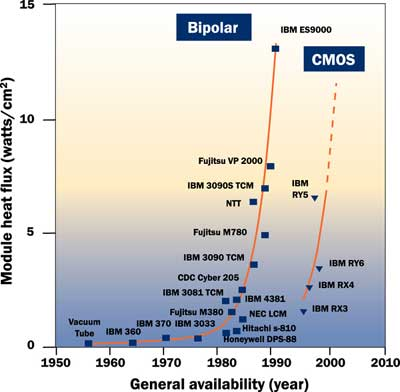
\includegraphics[width=0.9\linewidth]{Images/bipolarcmos.jpg}
\caption{Trends in module level power density, reproduced from \cite{chu:1999aa}. Copyright 1999 IEEE.}
\end{figure}
This pattern of improving hardware until physical limits force a switch to new technologies is a recurring one. The previous iteration saw widespread adoption of multi-core architectures, and once again we find ourselves encountering the limitations of this approach \cite{esmaeilzadeh:2011aa}. Unfortunately,  this time there is no mature semiconductor technology or transformational architectural paradigm waiting in the wings. Researchers are therefore searching for alternative ways to combat the rise of power consumption whilst we await the emergence of the next fundamental shift in processor technology. \golden

System architects are already focussing on power efficient chip design, with recent innovations in areas including on-die voltage regulation \cite{burton:2014aa}, Dynamic Voltage and Frequency Scaling (DVFS) scheduling \cite{kwon:2013aa} and energy efficient heterogeneous cores~\cite{gupta:2012aa}. Software engineers are also beginning take note of this issue as it becomes an increasingly pressing concern for scientific computing. \golden

The power draw of CMOS chips can be split into distinct components, the most significant of which are dynamic power and leakage power. Dynamic power is essentially the power consumed as logic gates change state while a processor performs work. Leakage power dissipation stems from the fact that at very small scales the insulating properties of silicon break down, allowing some current to flow (or leak) even when gates remain inactive. Other forms of power dissipation exist, however their effects are relatively minor. \golden

\begin{equation}
\label{eq:totpwr}
P_{tot} = P_{dyn} + P_{leak} + P_{other}
\end{equation}
\begin{equation} 
\label{eq:dynpwr}
P_{dyn} \propto CV^{2}Af
\end{equation}
\begin{equation}
\label{eq:leakpwr}
P_{leak} \propto V\left(ke^{\frac{-qV_{th}}{ak_{a}T}}\right)
\end{equation}

Equations~\ref{eq:dynpwr} and \ref{eq:leakpwr} above give relations for dynamic and sub-threshold leakage power respectively. In Equation~\ref{eq:dynpwr}, C denotes load capacitance (a property influenced by wire lengths of on-chip structures), $V$ the supply voltage, $A$ the activity factor and $f$ the clock frequency. Most of these terms are properties of the processor itself, however $A$ loosely equates to processor workload. Finally, the $V$ and $f$ terms are linked and vary in tandem as higher clock frequencies require higher supply voltages to sustain them. \golden

Equation~\ref{eq:leakpwr} is a simplified equation for sub-threshold leakage power. The new terms introduced in this equation include $T$, temperature, $V_{th}$, the transistor threshold voltage and $k$ the Boltzmann constant. The remaining parameters $q$, $a$ and $k_{a}$ capture CMOS logic design and fabrication characteristics. This is only one of several kinds of power leakage, however they all share the fact that they do not directly depend on processor workload. This means they are out of scope for software optimization and their details can be omitted.

An important feature of the equations governing power draw is that only $P_{dyn}$ is directly influenced by software, in particular due to its inclusion of the $A$ term. Software can also indirectly effect both dynamic and leakage current if it triggers changes to clock frequency and therefore supply voltage through DVFS. \golden

Historically, dynamic power has been the biggest contributor to $P_{tot}$, however leakage power has been on track to overtake it since the breakdown of Dennard Scaling.  Sub-threshold and gate-oxide leakage dominate total leakage current, and they both increase exponentially as transistors shrink. Process improvements like the introduction of high-k dielectric materials~\cite{jan:2009aa} have kept leakage power in check over the last decade, however there is no avoiding the fact that insulating properties will degrade as transistors get smaller. \golden

The final thing to consider in this section is the choice of metric to use when optimizing code. Energy is defined as the integral of power and time, so power may seem the natural metric to complement runtime techniques. This metric should be avoided, however, as it fails to consider the runtime implications of any code changes. Paradoxically, optimizations to reduce power draw can lead to increases in runtime and in turn greater total energy consumption.

Energy to completion is often chosen when energy consumption is of critical importance. It is often used in domains like mobile robotics where available energy is severely restricted. That said, in most domains energy is not the only limiting factor. In practice the most useful metrics are those which combine the effects of both energy and runtime. The simplest of these is the energy-delay product (EDP) \cite{gonzales:1995aa}, which assigns an equal weighting to both runtime and energy consumption. EDP can be defined in various equivalent ways:\golden

\begin{equation}
EDP = Energy \times Runtime
\end{equation}
\begin{equation}
\label{eq:edp}
EDP = Power \times Runtime^{2}
\end{equation}

Several variants of EDP have been proposed which assign greater weight to the runtime component in accordance with the demands of high performance computing. Common examples include energy-delay-squared product ($ED^{2}P$) and energy-delay-cubed product ($ED^{3}P$). We refer to this as the $E^mD^n$ family of metrics, which also includes simple power ($E^1D^{-1}$), energy ($E^1D^0$) and time ($E^0D^1$) as members. It can be argued that that $ED^{2}P$ is most suited when considering a fixed micro-architecture \cite{brooks:2000aa}, however our work applies to all members of this group with $M > 0$.

\section{Quantifying Power Optimizations}
\label{sec:quantifying}

We consider two related issues in the practical component of our work. The first task is to establish bounds on how much CPU power draw can vary whilst running arbitrary code. This allows us to place an upper limit on how much is possible to optimize a given code by. These bounds also help us tackle a second issue - namely to provide an objective appraisal of the power models proposed elsewhere in the literature.

The only relevant property an engineer can influence while optimizing software for reduced power consumption is activity factor. As previously discussed, the activity factor of a processor has a linear relationship with dynamic power and secondary non-linear relationships with both static and dynamic power. A developer wishing to save energy should therefore aim to modify their code to reduce its contribution to activity factor.

Although activity factor is defined as a scalar between zero and one, we know that in practice its range will be more limited. Many logic elements are dedicated to unavoidable tasks which involve frequent state changes, the most obvious being the propagation of clock signals. Conversely, we know that processors are not able to keep all their functional units active simultaneously. We therefore define the range of values that activity factor can feasibly take whilst running a code as $[\alpha  .. \beta]$ where $0 < \alpha < \beta < 1$.

From equations \ref{eq:totpwr}-\ref{eq:leakpwr} we know that, for a fixed platform and temperature, activity factors $\alpha$ and $\beta$ will be associated with constant power draws $P_{\alpha}$ and $P_{\beta}$ respectively, where $P_{\alpha} < P_{\beta}$. The values of these terms are naturally system-dependent and should be determined empirically. 

We are now ready to derive our visual heuristic to guide optimization. We begin by plotting lines with gradients $P_{\alpha}$ and $P_{\beta}$ in \figurename~\ref{fig:pow} to establish a feasible performance envelope. This represents the set of all $(P_{opt}, t_{opt})$ pairs for which $P_{\alpha}~<~P_{opt}~<~P_{\beta}$, with no bounds placed on runtime, $t_{opt}$. It should be clear that all codes,  and by extension their maximally-optimized equivalents, must be represented somewhere within this envelope.

\begin{figure}[ht]                                                               
\centering                                                                      
\lstset{basicstyle=\ttfamily\footnotesize\bfseries,                             
      frame=tb}                                                                 
\lstinputlisting[]{Listings/nops.c}                             
\caption{Baseline Power Benchmark}                            
\label{fig:nopjmpres}                                                           
\end{figure}  

We approximate $P_{\alpha}$ by monitoring the power consumed whilst running the code given in \figurename~\ref{fig:nopjmpres}, which effectively performs no work. It is safe to assume that this benchmark has a lower activity factor than a non-trivial code on any reasonable platform. We defer measurement of $P_{\beta}$ for now as its precise value is not relevant to the current discussion.

To constrain our search further we consider the metric we wish to reduce. We know that for two logically equivalent codes $a$ and $b$, the transformation $a \to b$ is a valid optimization with respect to a cost metric $M$ if and only if $M(a) > M(b)$. We plot the curve linking all points $b$ within our envelope where $M(a) = M(b)$. By definition, any valid optimization can only exist below this line. The exact equation of this curve varies depending on $M$, but can be found through basic algebra. For $ED^{2}P$ we get $y = (P_{a} \times t_{a}^{3}) / x^2$

Our final bound considers what it means to optimize code for reduced power draw. Our definition should be flexible enough to include optimizations which deliver significant reductions in power draw with minuscule reductions in runtime. On the other hand, we must avoid being too lenient. A large reduction in runtime associated with a negligible reduction in power draw should be regarded as a classical optimization.

Although this distinction may seem somewhat academic, it is an important consideration when searching for optimizations. In general, when the performance penalty is bigger in one domain than the other then intuitively the tools and techniques developed for that domain are better suited to finding the optimization.
\begin{figure}
 
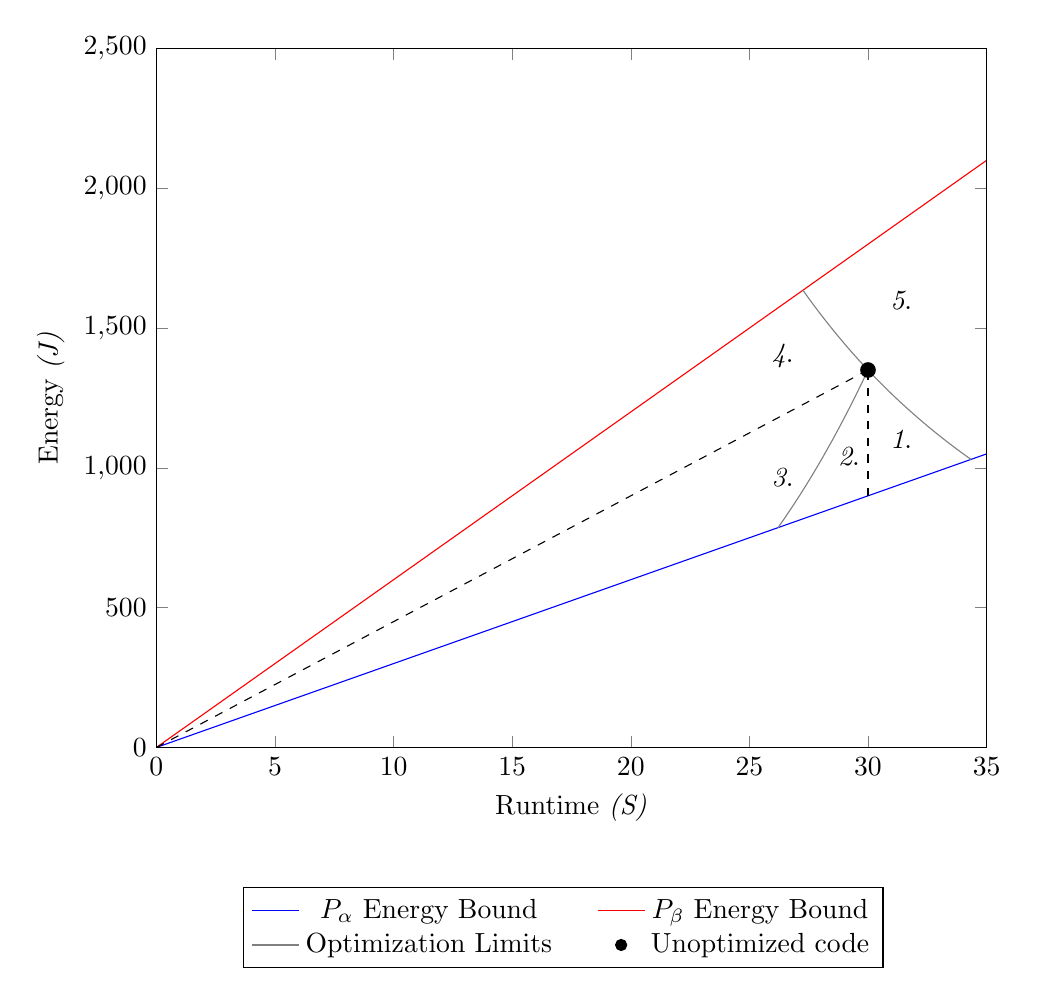
\begin{tikzpicture}
  \begin{axis}[no markers, ylabel={Energy \emph{(J)}}, xlabel={Runtime \emph{(S)}}, axis on top,
    ymin=0, ymax=2500,
    xmin=0, xmax=35,
    width=\linewidth,
    legend style={at={(0.49,-0.2)}, anchor=north,legend columns=2, /tikz/every even column/.append style={column sep=0.5cm}}
    ]

    \pgfmathsetmacro{\baseline}{30}
    \pgfmathsetmacro{\roofline}{60}
    \pgfmathsetmacro{\power}{(\baseline + \roofline) / 2}
    \pgfmathsetmacro{\seconds}{30}
    \pgfmathsetmacro{\energy}{\power * \seconds}
    \pgfmathsetmacro{\baseenergy}{\baseline * \seconds}


    \addplot[domain=\pgfkeysvalueof{/pgfplots/xmin}:\pgfkeysvalueof{/pgfplots/xmax}, blue] {\baseline * x};
    \addlegendentry{$P_{\alpha}$ Energy Bound} 


    \addplot[domain=\pgfkeysvalueof{/pgfplots/xmin}:\pgfkeysvalueof{/pgfplots/xmax}, red] {\roofline * x};
    \addlegendentry{$P_{\beta}$ Energy Bound}

    %ED2P boundaries
    \addlegendentry{Optimization Limits} 

    \addplot[domain=27.25680:34.34143, gray, forget plot] { (\power * \seconds^3) / ((x)^2)};
    \addplot[domain=26.2074:\seconds, gray] { (\power / \seconds^3) * x^4}; % Power time same ratio

    \addlegendimage{only marks, mark=o}
    \addlegendentry{Unoptimized code}


    \addplot[domain=\pgfkeysvalueof{/pgfplots/xmin}:\seconds, dashed] {\power * x};
    \draw[dashed] ({axis cs:\seconds,0}|-{axis cs:0,\baseenergy}) -- ({axis cs:\seconds,0}|-{axis cs:0,\energy});

    \node[circle,fill,inner sep=2pt] at (axis cs:\seconds,\energy) {};
    \node at (axis cs:31.4,1100) {\textit1.};
    \node at (axis cs:29.2,1040) {\textit2.};
    \node at (axis cs:26.4,965) {\textit3.};
    \node at (axis cs:26.4,1400) {\textit4.};
    \node at (axis cs:31.4,1600) {\textit5.};
      
 \end{axis}
\end{tikzpicture}

\caption{Optimization Classifications}\label{fig:pow}
\end{figure}

% All else being equal, energy to solution will reduce if a code can be made to run faster. That said, there is a clear difference between an optimization which specifically targets energy efficiency and this inevitable side-effect of classical optimization.

The definition we have settled on is that the transformation $a \to b$ is a valid power optimization w.r.t a metric $M$ if it is a valid optimization w.r.t. $M$ and the reduction in power draw has a greater impact on improvement in $M$ than any reduction in runtime. Once again, we plot the curve where both two factors have equal effects. All valid power optimizations must lie below this bound.

By plotting the various limits described above we subdivide the performance envelope into three distinct areas corresponding to power optimizations, time optimizations and degraded performance. For the purposes of illustration we add lines of constant time and energy allowing us to subdivide the plot further into the areas labelled:
\begin{enumerate}
\item Power-only optimizations
\item Power-mostly optimizations
\item Time-mostly optimizations
\item Time-only optimizations
\item Code degradation
\end{enumerate}

Between them, areas 1 and 2 represent the section of the performance envelope within which power optimization tools are most capable of identifying potential optimizations. Conventional tools should be used when trying to identify optimizations outside this area. The only parameters required to delineate this space for a given code are values for its runtime and energy costs and knowledge of system baseline power.

Despite its simplicity, this technique offers a surprising wealth of information. Figure \ref{fig:modelpoints} shows the power optimization area we observed when we ran the CFD benchmark of the Rodinia benchmark suite.


\begin{figure}
\label{fig:modelpoints}
 
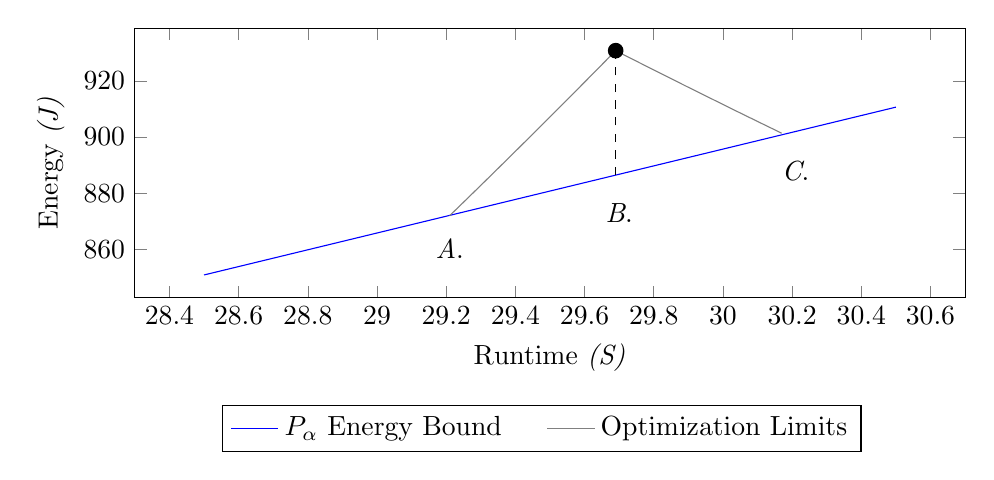
\begin{tikzpicture}
  \begin{axis}[no markers, ylabel={Energy \emph{(J)}}, xlabel={Runtime \emph{(S)}}, axis on top,
    width=\linewidth,
    height=5cm,
    legend style={at={(0.49,-0.4)}, anchor=north,legend columns=2, /tikz/every even column/.append style={column sep=0.5cm}}
    ]

    \pgfmathsetmacro{\baseline}{29.857} % NOP code

    %code, power, time
    %cfd, 31.348872, 29.689872
    %heartwall, 32.072718, 24.456485
    %lavaMD,  32.715703, 65.387028
    %leukocyte, 30.771108, 38.950881
    %streamcluster, 32.192283, 33.801999


     \addplot[domain=28.5:30.5, blue] {\baseline * x};
     \addlegendentry{$P_{\alpha}$ Energy Bound} 

  
     %% CFD %%
     \pgfmathsetmacro{\cfdpower}{31.348872}
     \pgfmathsetmacro{\cfdtime}{29.689872}
     \pgfmathsetmacro{\cfdenergy}{\cfdpower * \cfdtime}
     \pgfmathsetmacro{\baseenergy}{\baseline * \cfdtime}
     \addplot[domain=\cfdtime:30.17, gray, forget plot] { (\cfdpower * \cfdtime^3) / ((x)^2)};
     \addplot[domain=29.21:\cfdtime, gray] { (\cfdpower / \cfdtime^3) * x^4}; % Power time same ratio

     \node[circle,fill,inner sep=2pt] at (axis cs:\cfdtime, \cfdenergy) {};
     \addlegendentry{Optimization Limits} 

    \draw[dashed] ({axis cs:\cfdtime,0}|-{axis cs:0,\baseenergy}) -- ({axis cs:\cfdtime,0}|-{axis cs:0,\cfdenergy});
    
    \node at (axis cs:29.21,860) {\textit A.};                                   
    \node at (axis cs:29.7,873) {\textit B.};                                   
    \node at (axis cs:30.21,888) {\textit C.};                                   



%     %% CFD %%
%     \addplot[domain=39:48, gray] { (\sedtargetenergy * \sedtargetseconds *  \sedtargetseconds) / ((x)^2)};
%     \addplot[domain=33:41, gray] { (\sedtargetpower / \sedtargetseconds^3) * x^4}; % Power time same ratio
%     \addlegendentry{$ED^{2}P$} 
 

    
      
 \end{axis}
\end{tikzpicture}

\caption{Power Heuristic for Rodinia CFD}
\end{figure}

	
	
\todo{Working point}

We first construct a power model in the vein of those proposed in the literature. We then try to link the predictions of our model to the power equations given previously. Essentially we are attempting to test against the null hypothesis - to show how much better or worse our regressed model is better than a naive attempt.


\fragment{this tent shaped region}
\fragment{Despite its simplicity, this simple model provides us with lots of information. \todo{biggest gain to be had by using power vs classical optimization, energy reduction possible through power optimization ignoring any runtime effects, the maximum amount of time we can trade for any gains in energy efficiency, and a convenient way of comparing different codes}}




\fragment{Often power models are assessed by their performance relative to a measured baseline. Although this is important, this figure is somewhat meaningless without context. Our approach is one of quantifying 


\todo{Make this bit less attacky:}
It is also worth noting that this model is effectively useless from a code optimization standpoint as it does not take any software features into account. This property is intentional, as it allows us once again to provide a baseline from which to assess any models. One can only realistically expect to optimize a code to the level at which any changes can be accurately measured. A model which claims to assist in the optimization of codes can only offer optimizations to the extent it shows divergence from this baseline.

}


\fragment{The unknown quantities in our simplified power equations can be empirically measured. \todo{Occam's razor - stronger than regression if not out performed by it}}



\fragment{Accuracy figures without context are notoriously unreliable. To compensate for this we compare the outputs of various models against a baseline we have devised. This baseline consists of what we regard as the simplest non-trivial power model conceivable. This model stands in as a sort of null hypothesis test, our justification being that a complex model only adds value to the extent with which it outperforms this toy model.}

\fragment{Our toy model is not the simplest model possible - It is well established and readily apparent that runtime is the largest contributory factor to power consumption. One could therefore imagine a simple power model}

\fragment{We consider this to be the absolute minimum power consumption possible.}

\fragment{Intentionally simplistic. Our decision to simplify activity factor to active cores is part of this. We assume that instruction pipe-lining does a reasonable job of keeping as much silicon active as possible, and we do not know how much area an individual instruction activates, and a large percentage of power use is from clock circuitry anyway}



\fragment{Two components to our investigation. Firstly, the upper bound imposed by the baseline power consumption. Secondly, as we can only view power figures approximately, the error introduced into these models necessarily limits their usefulness as optimization tools beyond a certain point.}



\begin{table}


\centering
\small
\begin{tabular}{@{}ccccc@{}} \toprule
&\multicolumn{4}{c}{CPU Cores Active} \\ \cmidrule(r){2-5}
Frequency (GHz) & 1 & 2 & 3 & 4 \\ \midrule 
1.60 & 9.180 & 10.970 & 12.832 & 14.555 \\ 
1.70 & 9.449 & 11.446 & 13.295 & 15.112 \\ 
1.80 & 9.592 & 11.654 & 13.617 & 15.682 \\ 
1.90 & 9.816 & 12.009 & 14.168 & 16.291 \\ 
2.10 & 10.272 & 12.709 & 15.161 & 17.605 \\ 
2.20 & 10.559 & 13.161 & 15.705 & 18.333 \\ 
2.30 & 10.812 & 13.551 & 16.419 & 19.070 \\ 
2.40 & 11.303 & 14.290 & 17.012 & 19.946 \\ 
2.50 & 11.680 & 14.784 & 18.000 & 20.837 \\ 
2.60 & 11.819 & 15.144 & 18.616 & 21.879 \\ 
2.70 & 12.205 & 15.830 & 19.379 & 22.940 \\ 
2.90 & 13.095 & 17.196 & 21.155 & 25.344 \\ 
3.00 & 13.547 & 18.160 & 22.210 & 26.759 \\ 
3.10 & 14.048 & 18.870 & 23.639 & 28.284 \\ 
3.20 & 14.504 & 19.726 & 24.940 & 29.857 \\ 
\bottomrule
\end{tabular}
   \vspace{0.5\baselineskip}
\caption{Test Platform Base CPU Power (W)}
\label{tab:baseline}
\end{table} 



\todo{table 2 - benchmark results. Linpack is 35.2428 for 100 seconds}
\todo{Something about how any delta is about how the code uses more logic elements than our NOP lo ops. Our optimization window is therefore within that Delta}

\todo{Be nice, say that this does not invalidate other work, but simply shows that hardware has now reached \reword{convergence} and basically there's little traction left}

Having shown that 

\fragment{This model is not supposed to be rigorous or precise. Rather we present it as the simplest possible non-trivial power model which accounts for the sources of variability in the power equations. In effect our model is functionally equivalent to the power equations
presented previously with appropriate constants substituted \todo{sampled}. We present this model as our null hypothesis - for a model to be useful it must outperform this one. It is necessarily an oversimplification - it ignores clock gating. It should also consistently underestimate the true value, as the benchmark selected intentionally exercises the minimum possible number of logic elements while still performing work.}


\todo{One limitation of this work stems from the nature of RAPL - it is an accumulative measurement of power taking into account all processes. On a loaded system it will measure all tasks }

\begin{figure}
\label{fig:dummy_model}
\includegraphics[width=0.9\linewidth]{./Plots/dummy_model/dummymodel-figure0.pdf}
\caption{Feasible Performance Envelope}
\end{figure}

\todo{Decompose the model - find baseline vs non-baseline components}
\todo{This kind of shows us that the baseline dominates}

\fragment{Limitations to optimizations - the superfluous and the logical equivalences. The first is a no-brainer and boils down to removing unnecessary pre-fetching}

\fragment{Either optimizations which are off the critical path, or else those which are on the critical path }

\fragment{Put another way, any optimization which trades runtime for power has a limited window of}

\todo{equationify fact that energy is power * time, and assume we have power decreases, time static or increases}
\todo{equationify baseline lt optimized lt unoptimized lt roofline} \todo{note - roofline is tdp max}

\todo{Do maths think - by what margin would power have to go down to justify longer runtime? ratio of cost per watt, amortized cost per second}

Nothing discussed so far precludes power optimization in practice.
\todo{imply limits thus far are theoretical}
Even these tight limits may still admit some benefits at extreme scale.
Our final argument however is strictly economic.
\reword{A great deal of attention is paid to the fact that power costs are approaching parity with machine construction costs.} The \choice{implicit, unspoken} \choice{consequence, corollary, implication} being that this has not yet happened. \todo{Ultimate point being here the price difference, machine vs power cost places a further limit on optimization utility. Even if we manage to find a slower, more power efficient method of computing a given result, the cost of energy saved has to be less than the added amortized runtime cost.}


\todo{Legitimate targets for optimization: removing redundant prefetch operations as per phi paper.}

\section{Results}
\section{Review of Prior Art}
\label{sec:prior}

In this section we detail previous work which investigates the impact of software on power consumption. A wealth of material also exists on architecture-level power optimization, however this is outside the scope of our study.\golden

The ability to accurately measure a property is required in order to optimize for it. That said, reliable figures for power consumption are hard to obtain because complex hardware is required to measure instantaneous current at high temporal and currency resolutions. Several approachees  While each approach has its merits, not all are feasible tools for the average software engineer. Analytical Modelling and Architectural Simulation are both not suitable for this use case because they rely on intimate knowledge of the underlying hardware platform and are not 



This leaves us with Activity Factor Estimation and  Direct Measurement to concider.

\todo{Analytical Modelling, come up with a descriptive model of cpu and work stuff out.}

\todo{Architectural simulation - this works out the value for C for a target architecture. Find this bit in the book because it's well written.}

\todo{Activity Factor Estimation}

\todo{Direct Measurement - good because of accuracy, not useful because out of scope for average developer. powermon2.}


Architectural models can offer a breakdown of energy consumption by architectural block, but their results are difficult to relate back to software. They also rely on a detailed knowledge of processor internals which is seldom in the public domain. Instruction-level approaches measure average energy per instruction (EPI) figures to model processor energy. This approach yields results which are easier to relate to software, however it does not provide the same insights about the underlying sources of power consumption.\golden


Out of the options above, we conclude that the most applicable for use is an instruction level energy model based on activity factor estimation. This approach has been explored by a number of different groups in various ways. An \reword{archetypal} example is found  \todo{This is the example Power Prediction for Intel XScale Processors Using Performance Monitoring Unit Events}







\todo{tear this apart: Energy Measurement and Prediction for Multi-threaded Programs. 
The deviations usually lie below 10%
}


\todo{
\begin{itemize}
\item Measurement vs modelling Power is the integral and hard to measure
\item Approaches to measurement
\end{itemize}
}


\todo{Make sure to make the point that the accuracy quoted for models hovers around the same amount and is usually quoted as a simple average. There are several problems with such a figure. The simplest issue is that if a model can both over- and under-estimate, a low average error can be observed even when individual predictions are way off. If we give the authors the benefit of the doubt and assume they are reporting mean absolute error values. Even then, this methodology is somewhat flawed. To state a model yields an average error of 5\% does not necessarily display how good a model is. The nature of power, with both static and dynamic components along with known bounds means that reasonable guesses to power draw can be made a-priori. Any model constructed only has merit in as much as it beats these naive predictions.} 


\section{Conclusions}

\todo{IN an intuitive sense the covariance between these two signals, namely power and time consumption, is prohibitively high. The window of optimization exists in the ...word meaning freedom/decoupled component/... window}

\section{Shadow}

\todo{\begin{enumerate}
\item Merge this delta section - use for snippets
\item Consider a background section
\item Consider moving Code optimization out of intro
\item Write up power equations
\item Find recent source for percentage amount $P_{dyn}$
\item Are we limited to $P_{dyn}$?Think so
\item Optimizable range is only a small part of this part
\item Write a clear limitations section

\end{enumerate}
}



Architectural power reduction techniques focus on decreasing each of these terms.
For the purposes of software optimizations, however, we are limited to the dynamic power term, $P_{dyn}$, as this 

\reword{Common power reduction techniques
are based on architectural, logic or circuit design methods, decreasing f , AFi,
N or Vi [Zang et al. 2000; Hsieh and Pedram 2000; Shang et al. 2002]. TAKEN FROM Timing-Aware Power-Optimal Ordering of Signals}



\todo{Check this when book arrives}


\todo{STOLEN:
S. Kaxiras and M. Martonosi, Computer Architecture Techniques for Power-Efficiency, 1st ed. Morgan and
Claypool Publishers, 2008.

The end of Dennard scaling is expected to shrink the range of DVFS in future nodes, limiting the energy savings of this technique. This paper evaluates how much we can increase the effectiveness of DVFS by using a software decoupled access-execute approach. Decoupling the data access from execution allows us to apply optimal voltage-frequency selection for each phase and therefore improve energy efficiency over standard coupled execution.
}
\todo{Cite this paper for dennard: A 30 Year Retrospective on Dennard's MOSFET Scaling Paper}

\reword{Dennard scaling, which roughly, that as transistors get smaller their power density stays constant, so that the power use stays in proportion with area: both voltage and current scale (downward) with length \todo{cite Dennard's paper}}


 
% TODO should be an IEEE bibstyle or something
% Left because we don't know requisite format yet, but ho hum
\bibliographystyle{plain}
\bibliography{library}


\end{document}